\documentclass[border=10pt]{standalone}
\usepackage{tikz}
\usepackage{amsmath}
\usetikzlibrary{arrows.meta, positioning, fit, backgrounds, calc}

\begin{document}
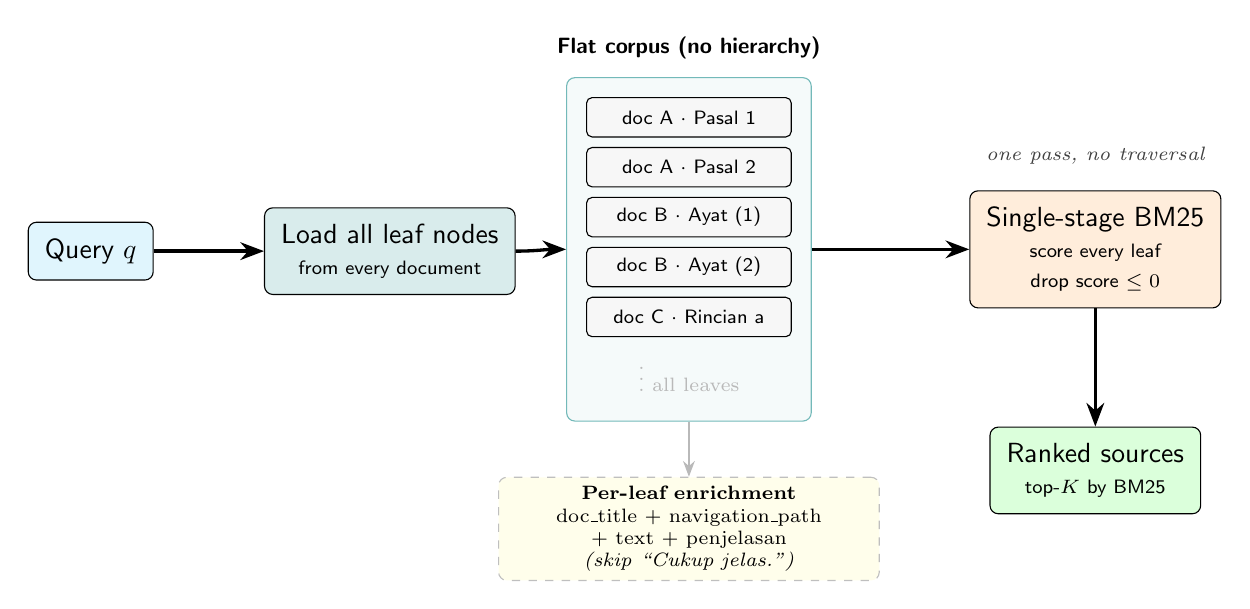
\begin{tikzpicture}[
    font=\small,
    box/.style={draw, rounded corners=3pt, align=center, font=\sffamily,
                inner sep=6pt},
    leaf/.style={draw, rounded corners=2pt, minimum width=2.6cm, minimum height=0.5cm,
                 font=\scriptsize\sffamily, align=left, inner sep=3pt, fill=gray!6},
    selleaf/.style={leaf, fill=orange!22, line width=0.8pt},
    flow/.style={-{Stealth[length=3mm]}, very thick},
    arr/.style={-{Stealth[length=2mm]}, semithick},
]

    %==================== QUERY ====================
    \node[box, fill=cyan!12] (q) {Query $q$};

    %==================== LOAD ALL LEAVES ====================
    \node[box, fill=teal!15, right=1.4cm of q, align=center] (load)
        {Load all leaf nodes\\[-1pt]{\scriptsize from every document}};
    \draw[flow] (q) -- (load);

    %==================== FLAT CORPUS (single pool, all docs) ====================
    \node[leaf] (c1) at ($(load.east)+(2.2,1.7)$) {doc A $\cdot$ Pasal 1};
    \node[leaf, below=0.12cm of c1] (c2) {doc A $\cdot$ Pasal 2};
    \node[leaf, below=0.12cm of c2] (c3) {doc B $\cdot$ Ayat (1)};
    \node[leaf, below=0.12cm of c3] (c4) {doc B $\cdot$ Ayat (2)};
    \node[leaf, below=0.12cm of c4] (c5) {doc C $\cdot$ Rincian a};
    \node[font=\scriptsize, text=gray!55, below=0.05cm of c5] (cdots) {$\vdots$ all leaves};

    \begin{scope}[on background layer]
        \node[draw=teal!55, rounded corners=3pt, fill=teal!4,
              fit=(c1)(cdots), inner sep=7pt] (corpus) {};
    \end{scope}
    \node[font=\sffamily\bfseries\footnotesize, anchor=south]
        at ([yshift=3pt]corpus.north) {Flat corpus (no hierarchy)};

    \draw[flow] (load.east) to[out=0, in=180] (corpus.west);

    %==================== ENRICHMENT note ====================
    \node[draw=gray!50, dashed, rounded corners=3pt, fill=yellow!8, font=\scriptsize,
          align=center, below=0.7cm of corpus, text width=4.6cm] (enrich)
        {\textbf{Per-leaf enrichment}\\
         doc\_title $+$ navigation\_path\\ $+$ text $+$ penjelasan\\
         {\itshape (skip ``Cukup jelas.'')}};
    \draw[arr, gray!55] (corpus.south) -- (enrich.north);

    %==================== SCORING ====================
    \node[box, fill=orange!14, right=2.0cm of corpus, align=center] (score)
        {Single-stage BM25\\[-1pt]{\scriptsize score every leaf}\\[-1pt]
         {\scriptsize drop score $\le 0$}};
    \draw[flow] (corpus.east) -- (score.west);

    %==================== TOP-K ====================
    \node[box, fill=green!14, below=1.5cm of score, align=center] (out)
        {Ranked sources\\[-1pt]{\scriptsize top-$K$ by BM25}};
    \draw[flow] (score.south) -- (out.north);

    %==================== single-stage emphasis ====================
    \node[font=\scriptsize\itshape, text=gray!50!black, above=0.2cm of score]
        {one pass, no traversal};

\end{tikzpicture}
\end{document}